% $Arbor$

\documentclass[10pt,twocolumn]{article}
\usepackage{times}
 
% includes and packages
\usepackage{wrapfig}                    %%% Wrap Text Around a Figure 
\usepackage{units}                      %%% Make Nice Fractions
%\usepackage{epsfig}                            %%% EPS figure support
\usepackage{cite}                       %%% improved citation support
\usepackage{supertabular}               %%% better table support
\usepackage{url}

%Check if we are compiling under latex or pdflatex
\ifx\pdftexversion\undefined
  \usepackage[dvips]{graphicx}
\else
  \usepackage[pdftex]{graphicx}
\fi

\clubpenalty=10000
\widowpenalty=10000
% need more space?
%\linespread{0.97}


% Set dimensions of columns, gap between columns, and paragraph indent
\setlength{\textheight}{8.875in}
\setlength{\textwidth}{6.875in}
\setlength{\columnsep}{0.3125in}
\setlength{\topmargin}{0in}
\setlength{\headheight}{0in}
\setlength{\headsep}{0in}
\setlength{\parindent}{1pc}
\setlength{\oddsidemargin}{-.1875in} % Centers text.
\setlength{\evensidemargin}{-.1875in}

% Add the period after section numbers. Adjust spacing.
\newcommand{\Section}[1]{\vspace{-8pt}\section{\hskip -1em.~~#1}\vspace{-3pt}}
\newcommand{\SubSection}[1]{\vspace{-3pt}\subsection{\hskip -1em.~~#1}
\vspace{-3pt}}

\begin{document}

\title{PhoneyC: A Virtual Client Honeypot}

\author{Jose Nazario\\jose@monkey.org}
% for two authors ...
%\author {\begin{tabular}[t]{c@{\extracolsep{8em}}c} 
%Jose Nazario  \\[1.5ex]
%        jose@monkey.org
%\end{tabular}}

\maketitle

\section*{Abstract}

The number of client-side attacks has grown significantly in the past few years, shifting focus away from defendable positions to a broad, poorly defended space filled with vulnerable clients. Just as honeypots enabled deep research into server-side attacks, honeyclients can permit the deep study of client-side attacks. A complement to honeypots, a honeyclient is a tool designed to mimic the behavior of a user-driven network client application, such as a web browser, and be exploited by an attacker's content. These systems are instrumented to discover what happened and how. This paper presents PhoneyC, a honeyclient tool that can provide visibility into new and complex client-side attacks. PhoneyC is a {\em virtual honeyclient}, meaning it is not a real application but rather an emulated client. By using dynamic analysis, PhoneyC is able to remove the obfuscation from many malicious pages. Furthermore, PhoneyC emulates specific vulnerabilities to pinpoint the attack vector. PhoneyC is a modular framework that enables the study of malicious HTTP pages and understands modern vulnerabilities and attacker techniques. 

\section{Introduction}
\label{intro}

Client-side attacks have radically changed the information security landscape in recent years. A significant portion of attackers in the past 20 years have focused on server-side goals and vulnerabilities. With two changes in the past few years, client-side attacks have become more successful for attackers. First, the web browser has become the de-facto tool to access Internet resources and is used for banking, communications, and every day life. To accomplish this, the web client has become more feature-rich and, in parallel, more complex, leading to many security vulnerabilities for attackers to exploit. Secondly, Internet servers have become significantly more hardened in the past 5 years than they were in previous years, significantly raising the bar for attackers to gain access. The client has become the weakest part of a network. This shift in the landscape has necessitated a change in exploit discovery and analysis.

An ever growing number of HTTP client-side attacks have been discovered and launched on the Internet~\cite{servers:kye}. In this time the complexity and sophistication of attacks has also grown, including obfuscation techniques and encryption, as well as server-side counter-surveillance techniques. Also in this time we have seen the appearance of exploit ``packs'' designed to facilitate the attacker's activities~\cite{provos:ayi}. These toolkits are able to construct dynamic HTML pages that encode many exploits into a single site in an attempt to infect the host. When coupled to massive website manipulations, these toolkits can infect thousands of PCs. 

One way of studying such toolkits is to use a client that is designed to be exploited so that the effects may be studied. We call such systems honeyclients~\cite{wang2005uhd}, a modification of the honeypot theme. Just as with honeypots, honeyclients can be high interaction to simulate all aspects of the client operating system, whereas a low-interaction honeypot only simulates the client application. We can also differentiate between real and virtual honeyclients. Real honeyclients use the actual application that would be attacked, whereas virtual honeyclients emulate the application in software. In this paper we refer to PhoneyC as a low interaction, virtual honeyclient because it only emulates the core functionality of a web client and no underlying OS features.

Virtual honeyclients are an attractive tool to use to study such content because they do not require additional computers to analyze vast amounts of malicious content and can easily scale. Using virtual honeyclients it is possible to inspect many websites in parallel with only one real system. However, to convince a website that it is talking to a legitimate client application we need to mimic the application's behavior and responses to inspection. 

This paper provides a brief overview of the design and implementation of PhoneyC, a client program that emulates a fully featured HTTP client. PhoneyC supports various client emulations, dynamic languages such as JavaScript, and mimics ActiveX add-ons, as well. PhoneyC can process a suspect web page and analyze the script bodies and react to the dynamic portions of the website. PhoneyC can be configured to mimic a variety of common web clients. 

To analyze the malicious content, obfuscated or encrypted JavaScript is decoded and reanalyzed, mimicking what the real web browser would do with such content. PhoneyC is the first virtual honeyclient that can perform dynamic analysis of JavaScript and Visual Basic Script to remove obfuscation. PhoneyC's virtual features are instrumented to understand their vulnerable functions and to provide alerts. Furthermore, downloaded content is scanned using an antivirus engine to look for known malicious content. PhoneyC can walk a malicious website and report on the exploit chain. We also provide an experimental evaluation of PhoneyC that shows that it can successfully decode and analyze exploit websites found in the wild. 

The rest of this paper is organized as follows. Section \ref{design} gives background information on PhoneyC's design and implementation. In section \ref{evaluation} we present an evaluation of PhoneyC in which we demonstrate its performance against real exploit sites found in the wild. Limitations of PhoneyC and virtual honeyclients are described in section \ref{weaknesses}. In section \ref{future-work} we discuss the limitations of the current PhoneyC design and discuss how it may be improved in the future. We provide related work in section \ref{related-work} and conclude in section \ref{conclusion}.

\section{Design and Implementation}
\label{design}

A virtual HTTP honeyclient is a combination of a web crawler and an analysis engine. Like a web crawler, it must be able to evaluate a web page and determine the links that lead out from the page. However, unlike a standard web crawler, it must be able to analyze the page to determine if it is malicious or benign. 

PhoneyC is implemented in the Python language~\cite{vanrossum2001plw} to aid in rapid development and extendibility, as well as integration with other tools and libraries. Python was also chosen to minimize security flaws that may appear in an implementation such as C or C++. At its core, PhoneyC has two major components: an input collector and an input evaluator. The input collector is simply a call to the Curl tool~\cite{ward2003clw} together with arguments to mimic a legitimate browser's behavior.

The basic requirements for PhoneyC are:
\begin{itemize}
	\item{PhoneyC must be able to convince a website that it is a legitimate web browser to collect the content that would be sent to an actual user.}
	\item{Second, PhoneyC must be able to enumerate all of the links from the HTML page and visit them. This includes all common HTML tags as well as generated HTML content, IFRAMEs, and redirections.} 
	\item{Third, PhoneyC must be able to understand and evaluate dynamic content such as JavaScript and Visual Basic Script. Fourth, PhoneyC must be able to detect malicious content and provide it for further analysis.} 
	\item{Finally, because PhoneyC is analyzing hostile code, it must be resilient to attacks itself.}
\end{itemize}

Basic data flow through PhoneyC is shown in Figure \ref{fig:phoneyc-flow}. URLs are fed to the system to initiate the evaluation, together with a referring URL when available (e.g. when a link is followed). The client retrieves the data using Curl from the server and stores all of the content on disk for additional analysis, if needed, and the data is scanned using an antivirus engine (ClamAV~\cite{kojm:ch}). Curl, running as a subprocess, provides a robust HTTP client in a separate process space, effectively as a sandbox to minimize client system attacks. 

If the content is HTML, the SGML parser collects the script content for JavaScript and Visual Basic Script (VBS). No restructuring of the input HTML (such as DOM validation or tag balancing) is performed which may alter the exploit. The parser also collects all of the outgoing links and normalizes them as needed. Links can be present as the common A and IMG tags, as well as IFRAME tags and redirects. The script bodies are analyzed as described below. The parsed page is stored as an object with all of its contents and attributes as a page object referenced by the origin URL. These attributes include the complete script bodies and all outgoing links. PhoneyC also understands major page events such as ``onLoad()'', but does not handle form submission or emulate mouse clicks. Once the full page has been analyzed, PhoneyC repeats the process for the next page with an outgoing link and the referring URL as inputs.

\begin{figure}[tb]
  \centering
  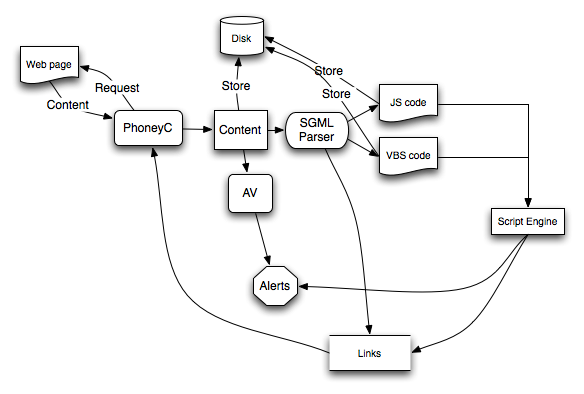
\includegraphics[width=\columnwidth]{pics/phoneyc_flow}
  \scriptsize
  \caption{Data flow within PhoneyC. One or more URLs are used to feed the client, which retrieves the content from the server. This is then stored on disk, scanned by AV for any suspect content, and also passed to an SGML parser for evaluation if it is HTML. The SGML parser breaks out script code by language for analysis by the specific script engine. The SGML parser also collects and normalizes any of the links from the HTML page as well as the output of the script output. Foreign scripts not included in the page, using the ``src'' argument to the SCRIPT tag, may also be collected and analyzed in the context of the current page. The script engines provide alerts to the system, as well.}
  \normalsize
  \label{fig:phoneyc-flow}
\end{figure}

PhoneyC is provided as a honeyclient module and an HTTP client script, ``honeywalk'', which calls the core methods of the honeyclient module. Honeywalk is demonstrated below. Other HTTP honeyclient tools can be build on the existing honeyclient module. 

PhoneyC is designed to crawl websites to discover exploits and also to act as a malcode collector. It is not, however, designed to extensively crawl the entire world wide web. As such, the scalability and speed deficiencies present in PhoneyC are not a pressing issue at this time. 

\subsection{Anti-Analysis Techniques}
\label{anti-analysis}

With the growth of web exploits has come a growth in their analysis. To bypass such analysis, attackers have begun applying obfuscation and encryption to their web exploit pages. This can make static analysis more challenging, but not impossible. In the past year we have seen more anti-analysis techniques appear that are designed to defeat illegitimate script access by tools such as PhoneyC. 

One of the major goals of PhoneyC was to ease the analysis of complex malicious websites. To do this, PhoneyC must be able to mimic a legitimate web browser to the server to receive the proper content, and to properly interpret the content to decode it. PhoneyC has been able to keep pace with most changes in the malicious website threat landscape, although some changes have been made during development. 

While some sites will send all exploit pages to all visitors, many sites will selectively direct clients to specific pages on the basis of their browser software. The following JavaScript differentiates between Microsoft Internet Explorer and other browsers, incorporating an IFRAME element with Internet Explorer-specific exploits if MSIE is found in the User-agent header. 
\scriptsize
\begin{verbatim}
if(navigator.userAgent.toLowerCase().indexOf("msie")>0)
  document.write("<iframe src=fl/ifl.html width=100 
                  height=0>");
else
  {document.write("<iframe src=fl/ffl.html width=100 
                   height=0>")}
\end{verbatim}
\normalsize
Obviously more sophisticated techniques to differentiate between browsers is possible. The User-agent header check may also be done on the server using, for example, a PHP script. 

To thwart such counter-analysis techniques, PhoneyC attempts to mimic a legitimate web surfer using a legitimate web browser. ``Personalities'' are created through the use of the User-agent header~\cite{bernerslee:htp} to mimic Internet Explorer 6 on Windows XP (the default) or Mozilla Firefox 2 on Windows XP. The JavaScript ``navigator'' object should also correctly mimic the client browser version. Other browsers may be mimicked through additional header forgery and script responses. Furthermore, if possible referring URLs are sent to the web server in the HTTP client headers, another check that some sites perform to ensure that only legitimate victims are served malicious content.

Once the content is presented by the server, additional measures may be in place to prevent detection by an external network-based tool such as an IDS or to slow down an analyst's inspection of the content. These sorts of methods often include variable name obfuscation or base-64 encoding of the content. More complicated techniques seen in the wild to thwart analysis may include:
\begin{itemize}
\item{Regular expression-based substitutions or removal of junk characters.}
\item{Compression of the script code, using an openly available script compressor that is popular in the web development crowd.}
\item{Encoding of the script code to provide some limited, basic encryption. We have seen more sophisticated sites use the page's URL as an encryption key, so that if the page is shared without the true URL it cannot be decrypted easily.}
\item{True encryption of the code using an encryption algorithm such as RSA.}
\end{itemize}
Additional methods have been seen and may be layered or repeatedly applied. Multi-stage encodings are not uncommon. The browser decodes one part of the page and uses the output of that part as a component of the script for the next part, such as a decoder routine. Some of these techniques have been adopted by attackers from existing, benign JavaScript protection tools and compressors, designed to optimize page load times~\cite{packer20}. 

% Anti-analysis tricks are an arms race and parallel the challenges facing Windows malicious binary analysis. In all cases, however, the script body must be executable by the browser, requiring it to be readable by a human, who can then perform analysis of it if needed.  

\subsection{Script Parsing}
\label{script-parsing}

Dynamic content in the form of JavaScript and Visual Basic Script is executed in a limited environment to perform dynamic analysis. JavaScript processing is done in a subprocess using the SpiderMonkey interpreter~\cite{foundation:sjc}. The web page's script body is collected and aggregated for analysis. A basic environment is prepended to the script body to mimic the browser's features, including the {\em document} object as well as {\em window} and the {\em navigator} object. Basic DOM inspection features, such as {\em getElementById} and others are implemented as well. 

Script obfuscation, very common in web page exploits~\cite{provos:ayi}, is bypassed with the script interpreter and some basic overrides in the script preamble. The ``eval()'' method, common to execute a newly decoded block of code, is overridden with a modified version that can recover if an error is observed by rerunning the script code with any of the output of previous runs. This effectively bypasses multi-stage decoders or decrypters where new code (e.g. a decrypter engine) is written to the page and then used in the next script interpretation. The modified version of  the ``eval()'' method then calls the real ``eval()'' method to get the proper result and prepends it to the script body as needed.

Visual Basic Script (VBS) code is analyzed using the vb2py package~\cite{vb2py} which translated VBS scripts into equivalent Python scripts. These scripts are then analyzed using a child Python interpreter process and the output is collected. The VBS subsystem is not yet as well developed as the JavaScript subsystem, but is designed to accomplish the same results.

\subsection{Vulnerability Modules}
\label{vuln-modules}

Detecting specific vulnerabilities to both classify them and to respond to them is a key design goal of PhoneyC. Rather than relying on external patterns or anti-virus alone which may not completely detect malicious HTML content, PhoneyC performs dynamic analysis of the content to determine the vulnerability and analyze the next action.

PhoneyC uses vulnerability modules to mimic vulnerable HTTP client extensions, including ActiveX controls and core browser functionality. These are similar to vulnerability modules in the MWCollect virtual honeypot~\cite{freiling2005bte} in that they are vulnerability-specific. However, unlike the MWCollect modules, they do not rely on matching shellcodes or patterns. Instead, these modules look for  exploit activity against a vulnerable method independent of the payloads. In a real browser, these objects are dynamically created in the script code and provide an interface between the browser and system libraries. In PhoneyC, these objects create pure JavaScript or VBS objects that implement core functional methods that are exploited. 

By using a virtual honeyclient and the vulnerability module architecture, PhoneyC avoids a number of real-world constraints. The primary challenge to discovering exploits on web pages with a real honeyclient is creating a vulnerable system. Often the necessary add-ons are not present. Another issue is the issue of language packs. In many cases an exploit is designed to work specifically on one Windows language pack but will not work on others. Virtual honeyclients can more quickly load more vulnerable modules than a real honeyclient, and they can analyze the exploit code for multiple language packs more easily.

An example vulnerability module, implementing checks for the WebViewFolderIcon.setSlice() attack (CVE reference ID CVE-2006-3730) is shown below. In this vulnerability, a magic value of 0x7ffffffe passed as the first argument to the ``setSlice()'' method enables arbitrary code execution by the attacker~\cite{setslice}. 
\scriptsize
\begin{verbatim}
function WebViewFolderIcon() {
    this.setSlice=function(arg0, arg1, arg2, arg3) {
        if (arg0 == 0x7ffffffe) {     // magic value
            add_alert('WebViewFolderIcon.setSlice attack');
        }
    }
}
\end{verbatim}
\normalsize
This JavaScript is one of many modules prepended to the page's JavaScript code that is analyzed by the system for any web page that includes script code. In this case the code looks for a magic value in the first argument to the setSlice() method and alerts when such code is found. Similar modules for other vulnerabilities can look for overly long arguments or arbitrary file access.

Creating new modules is relatively easy and requires two pieces, the vulnerability module and a reference to it via the ActiveX CLSID values. The module code itself simply creates a class and the appropriate methods and arguments together with argument inspection to determine when to alert. Furthermore, the modules can be written in the complete absence of any exploit code. All that is needed is to know the basics of the vulnerability, such as the method names and the nature of the malicious arguments, such as ``an argument longer than 400 bytes leads to a stack overflow''. Based on those conditions a simple argument scanner can be developed. The class is then referenced in the ActiveX map by the CLSID, both by hexadecimal values and by a simplified name. This provides a new HTML {\em object} is created, mapping the object ID and the CLSID to the right script class. 

Such an example is the NctAudioFile2 ActiveX control buffer overflow. A vulnerability description was used to create the vulnerability module, with analysis that reads in part~\cite{secunia:nctaudiofile}:
\begin{quote}
The vulnerability is caused due to a boundary error in the NCTAudioFile2.AudioFile ActiveX control when handling the ``SetFormatLikeSample()'' method. This can be exploited to cause a stack-based buffer overflow by passing an overly long string (about 4124 bytes) as argument to the affected method.
\end{quote}
Based on this description, the following vulnerability module was created:
\scriptsize
\begin{verbatim}
function NCTAudioFile2() {
   this.SetFormatLikeSample=function(arg) {
      if (arg.length > 4124) {
         add_alert('NCTAudioFile2 overflow in 
                    SetFormatLikeSample');
      }
   }
}
\end{verbatim}
\normalsize
Similar vulnerability modules can be written for exploits that use malicious object properties through the JavaScript ``watch()'' method, that handles property changes. The callback function to watch performs similar argument inspection to alert if an exploit scenario is encountered.

When an unknown CLSID is found, one for which PhoneyC has no modules, a message is generated. This can be used to develop new modules which may indicate their use in exploits. 

At this time over 65 unique vulnerability modules exist and are usable by PhoneyC. Major vulnerability modules include handlers for Yahoo Messenger, RealPlayer, and the WebFolderViewIcon handler in Internet Explorer 6. New modules are frequently added based on vulnerability reports and exploit code. 

\section{Evaluation}
\label{evaluation}

For a medium-scale evaluation of PhoneyC 470 unique URLs were gathered that were suspected drive-by download sites and web browser exploits. These URLs were gathered from various sites and materials including the URL blacklist maintained at lineage.paix.jp, the drive-by malware analysis blog at ilion.blog47.fc2.com, and the author's own suspect URL collection based on spam traps. URLs were submitted to the MITRE honeyclient system run by Honeyclient.org for analysis and also run through PhoneyC. The test system for PhoneyC was a MacBook running OS X 10.4.11 on an Intel Core Duo with a 2GHz clock speed and 2GB of SDRAM using Python 2.3.5 and SpiderMonkey 1.6. To speed up performance 24 PhoneyC processes were run in parallel. Each PhoneyC process was allowed a maximum depth of 4 links from the root URL. 

Of the 470 candidate URLs, 115 were live (yielding a 200 OK), 14 URLs yielded a 300-series redirect, 42 yielded an HTTP return code of 400 (a Bad request), 21 yielded a 401 (unauthorized) error, 149 yielded an HTTP 404 error (the URI was not found on the server), 269 were unreachable (the host was not responding), and the remaining sites' DNS names were unable to resolve. In total about 1.1MB of HTML text was downloaded and analyzed. 

\subsection{Performance}
\label{performance}

PhoneyC's performance is hampered by design weaknesses, including calling out to external processes such as Curl, ClamAV, and SpiderMonkey to assist with the analysis, as well as only working on one URL at a time. The 470 unique URLs analyzed in this evaluation data set provide a representative sample of PhoneyC's abilities. Some URLs were analyzed faster than others. URL evaluation took between 3 seconds at a minimum and over 3.2 hours at a maximum for any specific URL, depending on its complexity (number of outbound links and any encountered script evaluation time). The average URL took 2.1 hours to analyze all outbound links and script code at a maximum distance of 4 references, including images as well as links off of the page. Note that PhoneyC can be slowed down dramatically if the HTTP server for the URL is unreachable. 

In contrast, the MITRE honeyclient, in contrast, was able analyze the 470 URLs in approximately 14 minutes. This is due to using a native browser, working in even greater parallel, and only loading the one URL (including images and scripts) before leaving the URL. 

\subsection{Accuracy and Insights}
\label{accuracy}

From the 470 URLs, 22 unique HTML pages (unique via MD5 checksums) were downloaded, of which 2 yielded hits in ClamAV (both for the signature Exploit.CVE-2006-3730).  Other scanners tested included Kaspersky Antivirus, BitDefender, Grisoft's AVG, and Fortinet's `vscanner' tool, none of which yielded signature hits on the HTML downloaded by PhoneyC. Over 2700 script bodies were evaluated (through a series of dynamic evaluations by PhoneyC), only three of which yielded positive signature hits with ClamAV for JS.Dropper-33 and Exploit.HTML.IFrameBOF-4. 

Dynamic analysis by PhoneyC revealed that the most popular exploits found in the URL corpus were for the Xunlei Thunder 5.x DownURL2() overflow~\cite{xinlei} (6 found in total) and the PPStream (PowerPlayer.dll 2.0.1.3829) ActiveX Remote Overflow Exploit in the Logo property~\cite{pplayer:ex} (6 found in total in this data set). PhoneyC is able to emulate this ActiveX control that has been widely exploited as a malcode dropper. As described below, PhoneyC's limits means that it is unable to capture all exploits seen in the wild, however. 

In contrast to PhoneyC's findings, the MITRE honeyclient setup found only 4 URLs that registered an alert. These differences highlight weaknesses of PhoneyC as well as some of its strengths.

URLs that registered an alert in PhoneyC did not always register issues in the MITRE honeyclient setup. An example is the URL http://www.pineapple4u.com/relogonn.htm. This was flagged as containing an exploit in PhoneyC (Exploit.CVE-2006-3730) even though the JavaScript subsystem was unable to process the script correctly. This is due to the combined approach used by the tool to analyze URLs. 

Another example is the URL http://www.lineagecojp.com/tmsn/StormII.htm from the feed of URLs processed by both PhoneyC and the MITRE honeyclient. In this case PhoneyC's dynamic script analyzer found an issue with the page and flagged an exploit for the PPStream (PowerPlayer.dll 2.0.1.3829) ActiveX Overflow in the rawParse() method, even though ClamAV did not register an issue. The MITRE honeyclient did not flag this host. 

An example where both PhoneyC and the MITRE honeyclient agreed that a URL was malicious was with the root exploit URL http://sexbases.cn/in.cgi?16\&1dfcb2. This URL was flagged as suspicious by the MITRE honeyclient. PhoneyC is able to reveal that through a series of scripts and IFRAMEs the real exploit URL is http://dasretokfin.com/index.php, which exploits Exploit.CVE-2006-3730. 

PhoneyC missed some of the URLs flagged by the MITRE honeyclient, such as http://www.lineagecojp.com/ie/Ms06014.htm. In this case this is a commonly found exploit for an XML Request object in Internet Exploit 6. This emulation is not fully available in PhoneyC at this time, so the dynamic script analyzer was unable to correctly analyze this URL. Another URL missed by PhoneyC was http://freeonlinehostguide.com/index.php. The MITRE honeyclient correctly recognized an exploit on this page but PhoneyC was not able to fetch any HTML contents for this URL and so was not able to determine if the site was malicious. This is commonly due to poor emulation of the Internet Explorer request to a web server which looks for specific browser request features before serving the content. 

Hostname blacklists were also used to compare the findings and any suspicious nature of the URLs. If a domain name for the URL appears on a blacklist the URL itself may be malicious. To test this, and to verify that the URLs were possibly malicious, three blacklists were queried for the hostnames in the URLs. The results of any blacklisting are shown in Table \ref{blacklist}. 

\begin{table}
\centering
\begin{tabular}{r|r}
\hline
{\bf Blacklist domain} & {Number of domains blacklisted} \\
\hline
sophosxl.com & 83 \\
surbl.org & 102 \\
mailshell.net & 90 \\ 
\hline
\end{tabular}
\bigskip
\scriptsize
\caption{Number of URLs screened by PhoneyC blacklisted by major DNS-based blacklists. This indicates that these URLs are possibly suspicious based on the domain name status.}
\normalsize
\bigskip
\label{blacklist}
\end{table}
\section{PhoneyC Detection}
\label{weaknesses}

Virtual honeyclients are open to a number of detection techniques and attack vectors. A number of these issues are present in any virtual tool due to the limits of software emulation and will be present in any virtual honeyclient. 

PhoneyC specifically is vulnerable to detection through a simple check for the ``page\_alerts'' array in any of the JavaScript code. This variable name is not hidden at all and is accessible by any of the script code. A malicious page can simple check for the existence of this variable by reference and exit if it is found. To remedy this, the variable reference can be randomly generated, for instance.

As shown in the previous section, PhoneyC is also much slower than a normal web browser, enabling timing attacks to be used against it. This is an extension of a simple debugger check which uses the time elapsed between two set points to detect single stepping. A malicious server that measures the time between requests that should be very short can deny the client content. Performance improvements and concurrent requests to mimic a standard web browser would remedy this issue.

When impersonating Internet Explorer, PhoneyC can be detected through the SpiderMonkey JavaScript interpreter, which differs slightly from the script engine in the real Internet Explorer. Certain behaviors are well known and derive from ambiguities in the JavaScript specification, such as regular expression handling. Any virtual honeyclient that relies on SpiderMonkey will suffer the same issues. 

Finally, any virtual honeyclient will always fail to emulate all aspects of a real browser. Dynamic content can be used to inspect arbitrary features of the browser using calls that may not be documented. As such, suspicious sites may be able to detect virtual honeyclients by calling methods that are not implemented. This parallels attacks to detect virtual execution environments used in malware sandboxing~\cite{natvig:2008} and is a fundamental flaw of any kind of emulation.

\section{Future Work}
\label{future-work}

PhoneyC is far from complete at this point, although it is one of the tools the author uses to analyze malicious websites. Currently a number of factors are being evaluated to redesign PhoneyC to add functionality and improve reliability and performance. Minor improvements include easier configuration, proxy support, and performance enhancements. PhoneyC's vulnerability module architecture is being re-evaluated to handle previously unknown ActiveX CLSIDs and methods using a generic approach. Additionally, a generic scripting language framework is being developed to avoid having to write two vulnerability modules for any specific attack vector, one in JavaScript and one in VBS. Major PhoneyC deficiencies and improvements we are evaluating are listed below.

\subsection{Exploit Enumeration}
\label{exploit-enumeration}

One major drawback to the current design of the vulnerability modules is that they can only alert for a single exploit that the system knows of. All other vulnerabilities that may be present in the web page are not analyzed and not reported. The author previously developed a version of the script analysis engine used in PhoneyC, dubbed ``Norberto'', that performed static analysis of the page to enumerate multiple exploits in the page after some basic dynamic analysis to decode the page. In the future, PhoneyC may be extended with a similar static analysis engine to enumerate the complete list of exploits in the page.

\subsection{Additional Content Types}
\label{add-content}

Since PhoneyC was first developed, a number of new content types have become the focus of exploit activity, including Adobe's Portable Document Format (PDF) and their Flash format. These content types are not understood by the tool and may contain malicious content. Currently, we use manual techniques to analyze malicious Flash and PDF documents. Their increased use on the web as a means to deliver malicious executables to the end user means that we should incorporate their analysis into PhoneyC.

\subsection{Shellcode Analysis}
\label{shellcode}

PhoneyC is not able to understand shellcode that may be presented in the dynamic HTML page and is currently limited to a generic alert for a vulnerable method. Because of this, an analyst must still perform follow-up analysis of the content to determine the next stage of the attack. We have been working on integrating a shellcode analysis engine, libEmu~\cite{libemu}, into the dynamic payload inspection engine to further understand the next stage of the attack. This will also require tighter integration with the SpiderMonkey script engine. 

\section{Related Work}
\label{related-work}

Previous work at characterizing widespread web-based malware has been described by Provos {\it et al}~\cite{provos:gba}. In their work, ``drive by'' websites were found to be widespread and arising from website compromises and third-party script abuse, such as JavaScript-based visitor counters.

PhoneyC is not the first such honeyclient tool and builds on a number of previous works. The vulnerability module concept was inspired by the MWCollect virtual honeypot daemon~\cite{freiling2005bte}. In PhoneyC, modules are designed to mimic vulnerable ActiveX controls and implement the methods in JavaScript. Argument checks validate the input and provide a simple alerting mechanism. 

Seifert's HoneyC is a low interaction, virtual honeyclient tool~\cite{seifert2006hli}. However, it suffers from a lack of ability to analyze obfuscated dynamic HTML and reliance on Snort signatures for detection, which is easily evaded.

Real honeyclients have been developed by multiple independent groups. Seifert's Capture-HPC is a high interaction honeyclient~\cite{mara:chc} that can be used with, for example, Windows XP and Internet Explorer to analyze malicious websites. The MITRE HoneyClient uses Internet Explorer running on Windows~\cite{wang2005uhd}. Fed a list of URLs, the system will visit the URL if needed or pull the results from a local cache. When the URL is visited, if unexpected system changes occur, the URL is marked as suspicious and the new files are made available for additional analysis. The HoneyMonkey project is another large-scale, automated web crawling effort to discover malicious website~\cite{wang2006awp}. URLs are visited both by an older version of the browser and by a newer, up-to-date version to discover previously unknown and unpatched issues. Both are limited in their attack visibility as they require vulnerable modules to be installed in the client.

Not all honeyclient tools are restricted to HTTP content. The SHIELA honeyclient uses Outlook Express driven by external scripts to discover mail-based threats~\cite{rocaspana:sch}. Trigger conditions are very similar to those of the MITRE Honeyclient, namely an alert happens if one of a set of illegal operations occurs, such as Windows registry changes, file creation, or specific network traffic. 

Honeyclient research is also being done using browser plug-ins. Efforts are also underway to incorporate some of the basic heuristics and detection capabilities of honeyclients into real browsers used by analysts~\cite{hallaraker2005dmj}. 

\section{Conclusion}
\label{conclusion}

PhoneyC is a virtual honeyclient for analyzing websites. It mimics legitimate web browsers and can understand dynamic content, and is the first virtual honeyclient that can de-obfuscate malicious content for detection. By using vulnerability modules, specific attacks can be pinpointed and characterized much faster than with manual analysis. 

We gave an overview of PhoneyC's design and architecture and showed how PhoneyC's analysis engine understands malicious websites. Our experimental evaluation showed that PhoneyC works on current, in the wild malicious websites, albeit with room for improvements in both performance and features. We demonstrated that PhoneyC can determine what malicious software may be loaded onto a system if exploits exist. 

PhoneyC is publicly available as source code under a GNU Public License. The subversion repository is available at http://code.google.com/p/phoneyc .

\section*{Acknowledgments}
\label{acks}

I would like to thank Georg Wicherski for his review of this paper, his contributions to the PhoneyC codebase and his assistance in a re-design of the toolkit. I would also like to thank Marco Cova for helpful discussions and bugfixes with PhoneyC. Chris Lee, Adrian Wiesmann, David Watson, and Christian Siefert all provided a generous review of this manuscript.

\scriptsize
\bibliographystyle{abbrv}
\bibliography{phoneyc}
\normalsize

\end{document}

% mal sites under review for evaluation, mar 31 2009
%http://qwr1.cn
%http://forum.csrcentre-bd.org/	
%http://www.ranninp.com/001359/Ms06014.htm
%http://qjwm88.cn/02/02.htm
%http://www.qiqigm.com/04.htm
%http://hyrzqf.cn/06014.htm
%http://o7n9.cn/1.htm
%http://loveuswarters.cn/1.html
%http://q20080911.com.cn/1/04.htm
%http://q20080911.com.cn/1/14.htm
%http://www.worldofwarcrokft.com/1/Office1.htm
%http://www.dao-hang8.cn/10/06014.htm
%http://www.dao-hang8.cn/10/NCT.htm
%http://www.dao-hang8.cn/10/bfyy.htm
%http://www.dao-hang8.cn/10/f2.html
%http://www.dao-hang8.cn/10/flash.htm
%http://www.dao-hang8.cn/10/i1.html
%http://www.dao-hang8.cn/10/index.htm
%http://www.dao-hang8.cn/10/lz_new.htm
%http://www.dao-hang8.cn/10/office.htm
%http://www.dao-hang8.cn/10/real10.htm
%http://www.dao-hang8.cn/10/real11.htm
%http://www.dao-hang8.cn/10/sina.htm
%http://1818666.com/111/index.htm
%http://www.fdsfaf.cn/118.htm
%http://www.gsafs.cn/120.htm
%http://gt.kfjed.org.cn/14.htm
%http://www.goooog1e.cn/2.htm
%http://www.jhnbt.cn/31.html
%http://o7n9.cn/456.htm
%http://www.skjdhr.cn/54.htm
%http://fivecq.cn/65.htm
%http://google.nan7.cn/6666/link/06014.htm
%http://google.nan7.cn/6666/link/Uc.htm
%http://google.nan7.cn/6666/link/cx.htm
%http://google.nan7.cn/6666/link/ff.htm
%http://google.nan7.cn/6666/link/flash.htm
%http://google.nan7.cn/6666/link/index.html
%http://google.nan7.cn/6666/link/mi.htm
%http://google.nan7.cn/6666/link/real10.htm
%http://google.nan7.cn/6666/link/real11.htm
%http://google.nan7.cn/6666/link/xl.htm
%http://google.nan7.cn/6666/s1.html
%http://www.kiki02.net/7.htm
%http://loveuswarters.cn/7.html
%http://newymdt5.cn/85.htm
%http://333mas8d.cn/9/flink.html
%http://333mas8d.cn/9/ilink.html
%http://565duomayi.cn/9/sf.htm
%http://newymdg8.cn/92.htm
%http://www.88feel.cn/Bfyy.htm
%http://www.coconlovely.com/Blog/06014.htm
%http://www.bluewoon.com/Blog/0733.htm
%http://www.skywebsv.com/Blog/1.htm
%http://www.skywebsv.com/Blog/2.htm
%http://www.bluewoon.com/Blog/flash.htm
%http://www.bluewoon.com/Blog/index1.htm
%http://www.skywebsv.com/Blog/ms06014.htm
%http://www.bluewoon.com/Blog/real11.htm
%http://www.coconlovely.com/Blog/realplay.htm
%http://adlaji.cn/GLWORLD.html
%http://bakcss.cn/Lz.htm
%http://bakcss.cn/Main.htm
%http://www.88feel.cn/Ms06014.htm
%http://www.xlsf013.cn/Pps.htm
%http://adlaji.cn/Real.html
%http://hyrzqf.cn/Real10.htm
%http://user1.12-71.net/Real10.html
%http://adlaji.cn/Thunder.html
%http://asp-17.cn/UU.htm
%http://www.832821.cn/Webxls.htm
%http://www.fffffffggggg.cn/a0047129/Ms06014.htm
%http://www.fffffffggggg.cn/a0047129/a04.htm
%http://www.fffffffggggg.cn/a0047129/flink.html
%http://www.fffffffggggg.cn/a0047129/fx.htm
%http://www.fffffffggggg.cn/a0047129/ilink.html
%http://www.fffffffggggg.cn/a0047129/new.html
%http://asp-10.cn/a1/GLWORLD.html
%http://asp-10.cn/a1/Real.html
%http://asp-10.cn/a1/Thunder.html
%http://asp-10.cn/a1/flink.html
%http://asp-10.cn/a1/fx.htm
%http://asp-10.cn/a1/ilink.html
%http://asp-10.cn/a1/ms06014.htm
%http://asp-10.cn/a1/real.htm
%http://asp-10.cn/a1/ss.html
%http://sllwbd8.cn/a117/fxx.htm
%http://www.jsp369.cn/a22.htm
%http://asp-10.cn/a5/GLWORLD.html
%http://asp-13.cn/a5/Ms06014.htm
%http://asp-10.cn/a5/Real.html
%http://asp-10.cn/a5/Thunder.html
%http://asp-10.cn/a5/flink.html
%http://asp-10.cn/a5/fx.htm
%http://asp-10.cn/a5/fxx.htm
%http://asp-10.cn/a5/ilink.html
%http://asp-10.cn/a5/ms06014.htm
%http://asp-10.cn/a5/real.htm
%http://asp-12.cn/a5/ss.html
%http://asp-10.cn/a5/ss1.html
%http://asp-5.cn/a5/ss111.html
%http://bakcss.cn/a8.htm
%http://www.cao360cao.cn/aa2.htm
%http://www.fdsfaf.cn/abckkk.html
%http://jzm015.cn/ac.htm
%http://www.751down.cn/ad.htm
%http://www.111nv.cn/ad.html
%http://www.stats.dl.gov.cn/admin/activity/pic/index.htm
%http://www.jhnbt.cn/al.html
%http://www.118bi.cn/all/aa.htm
%http://www.118bi.cn/all/afl.htm
%http://www.118bi.cn/all/aho.htm
%http://www.118bi.cn/all/alz.htm
%http://www.118bi.cn/all/anrl.htm
%http://www.118bi.cn/all/bb.htm
%http://www.118bi.cn/all/new.htm
%http://www.tooplogui.com/asindex.htm
%http://www.1ovel.cn/asp/1.htm
%http://www.1ovel.cn/asp/as.htm
%http://www.1ovel.cn/asp/m6.htm
%http://www.kele88.com/av/help.htm
%http://ph.errtys.org/ax14.htm
%http://www.tongji123.org/axfs.htm
%http://ph.errtys.org/axlz.htm
%http://abca5.cn/b057850/b05.htm
%http://abca5.cn/b057850/new.html
%http://www.hxg001.cn/b5.htm
%http://bg.dcjsx.cn/baofeng.htm
%http://www.gamemmobbs.com/batteROyale/Ms06014.htm
%http://www.mabi360.cn/bb2.htm
%http://13n7.cn/bbs/flink.html
%http://web.do2a.cn/bbs/fx.htm
%http://vitas01.cn/bbs/gm.htm
%http://k3ks.cn/bbs/ilink.html
%http://17178bbs.cn/bbs/index.htm
%http://www.symphones.com/bbs/index1.htm
%http://wmnvasd4.cn/bbs/sina.htm
%http://www.bwirx.cn/bf.html
%http://www.puma166.com/bfyy.htm
%http://www.taikooo.cn/bk185.htm
%http://www.dosmov.cn/bk200.htm
%http://www.livedoorm.com/blog.htm
%http://www.atewikijp.com/blog/
%http://www.nicovideojps.com/blog/13n7.cn/bbs/ilink.html
%http://gt.fdnc.net.cn/bx14.htm
%http://gt.fdnc.net.cn/bxlz.htm
%http://www.832821.cn/c145.htm
%http://www.baibaiasd.cn/c4.htm
%http://www.maplestorfy.com/caink/caink.htm
%http://www.grandchasse.com/caink/lin.htm
%http://www.grandchasse.com/caink/rmtline.htm
%http://jerikoblog88fc2.com/category2-2.html
%http://kky66.cn/cc/z1.htm
%http://kky66.cn/cc/zz.htm
%http://user1.bwseo.cn/ce.htm
%http://229dj.cn/cn4.htm
%http://loskut.cn/cotton.html
%http://sexbases.cn/cow.html
%http://d.webdaa.cn/cuteqq.htm
%http://www.bbtv-chat.com/cuvt66895/Ms06014.htm
%http://www.webs600.cn/d1.htm
%http://222.189.239.3/d3/123.htm
%http://222.189.239.3/d3/zz3.htm
%http://ymcascaws9.cn/dao/a.htm
%http://ymvsanw16.cn/dao/d.htm
%http://www.gogo111.net/dl6.htm
%http://www.pang123.cn/e2.htm
%http://sexbases.cn/edit.html
%http://www.gamemmobbs.com/esports/Ms06014.htm
%http://www.bjhjjl.cn/ewebeditor/Ms06014.htm
%http://www.gamanir.com/exe/wm.htm
%http://gt.fdnc.net.cn/f.htm
%http://www.infosueek.com/ff11diary/index.htm
%http://www.k5dionne.com/ffxmmi/index.htm
%http://kk.jackkk.cn/fgame.html
%http://www.sunwayto.com/file/file.htm
%http://229dj.cn/flash.htm
%http://www.playenline.com/flash/flash.htm
%http://bczouhao.cn/flash/flink.html
%http://bczouhao.cn/flash/ilink.html
%http://17178bbs.cn/flash/index.htm
%http://www.gameicity.com/flash/zuo.htm
%http://user1.12-71.net/flink.htm
%http://d.webdaa.cn/flink.html
%http://www.falurl.com/flleo/usmmtupo.htm
%http://ageofconans.net/fsb/flink.html
%http://ageofconans.net/fsb/ilink.html
%http://ageofconans.net/fsb/index.htm
%http://jzm015.cn/fx.htm
%http://jzm015.cn/fxx.htm
%http://bakcss.cn/fzl.htm
%http://www.playonlanei.com/game/Ms06014.htm
%http://www.8568985.com/garegky/egk.htm
%http://www.fdsfaf.cn/ggbbyahoo.html
%http://www.pang357.cn/ghost.html
%http://www.awserk.cn/go.html
%http://ph.errtys.org/gol/am1.htm
%http://sexbases.cn/gr.php
%http://www.nifala01.info/hao104.htm
%http://web.fd5a.cn/hc/fh.htm
%http://loveuswarters.cn/hi.htm
%http://www.maplestorfy.com/holy_immortals/tals/ff.htm
%http://www.maplestorfy.com/holy_immortals/tals/ffn.htm
%http://www.maplestorfy.com/holy_immortals/tals/fftu.htm
%http://www.maplestorfy.com/holy_immortals/tals/index1.htm
%http://www.maplestorfy.com/holy_immortals/tals1/index2.htm
%http://www.maplestorfy.com/holy_immortals/tals1/mo.htm
%http://www.maplestorfy.com/holy_immortals/tals1/mu.htm
%http://www.maplestorfy.com/holy_immortals/tals1/nu.htm
%http://www.maplestorfy.com/holy_immortals/tals2/Ms06014.htm
%http://www.maplestorfy.com/holy_immortals/tals2/main.htm
%http://www.playonlino.com/home/Ajax.htm
%http://www.playonlino.com/home/Bfyy.htm
%http://www.playonlino.com/home/XunLei.htm
%http://wm66.8800.org/htm/06014.htm
%http://wm66.8800.org/htm/b1.htm
%http://wm66.8800.org/htm/bfyy.htm
%http://wm66.8800.org/htm/f2.html
%http://wm66.8800.org/htm/flash.htm
%http://wm66.8800.org/htm/i1.htm
%http://wm66.8800.org/htm/lzx.htm
%http://wm66.8800.org/htm/net.htm
%http://wm66.8800.org/htm/new.htm
%http://wm66.8800.org/htm/office.htm
%http://wm66.8800.org/htm/real10.htm
%http://wm66.8800.org/htm/real11.htm
%http://www.lineagecojp.com/ie/Ms06014.htm
%http://www.lineagecojp.com/ie/Ms06046.htm
%http://www.lineagecojp.com/ie/StormII.htm
%http://www.lineagecojp.com/ie/Xunlei.htm
%http://www.lineagecojp.com/ie/Yahoo.htm
%http://www.lineagecojp.com/ie/main.htm
%http://www.testinghua.com/ie/ragnarokonline/Ms06014.htm
%http://www.testinghua.com/ie/wm.htm
%http://www.xinluoqu.com/ied/index1.htm
%http://kk.jackkk.cn/igame.html
%http://user1.12-71.net/ilink.htm
%http://d.webdaa.cn/ilink.html
%http://www.imbbs2t4u.com/imbbs/imbbs.htm
%http://www.imbbs2t4u.com/imbbs/mbb.htm
%http://sexbases.cn/in.cgi?16&1dfcb2
%http://boaaa.3322.org/index.htm
%http://219.136.252.219/index.html
%http://freeonlinehostguide.com/index.php
%http://hostindianet.com/index.php?cocacola25
%http://hostindianet.com/index.php?cocacola26
%http://www.mbspro6uic.com/indexff.htm
%http://www.mbspro6uic.com/indexm.htm
%http://windows.loveyoushipin.com/ing/le.htm
%http://www.lineageinfo.com/injplink/inlink.htm
%http://www.fxfqiao.com/jp/jp.htm
%http://www.userlg.cn/jp20.htm
%http://www.woshijianren.com/jpjp/Ms06014.htm
%http://www.woshijianren.com/jpjp/jpro.htm
%http://www.fxfqiao.com/jpsk/love.htm
%http://www.dyyh.com.cn/ktm/2.htm
%http://www.knbyu.cn/l.html
%http://www.aspxia.com.cn/la03.htm
%http://loveuswarters.cn/le.htm
%http://www.oulianyong.com/lin240/index.htm
%http://rmtfane.com/link179700/Ms06014.htm
%http://www.nlftweb.com/link179700/index.html
%http://www.zgynkmq.cn/llsg/5.htm
%http://hostindianet.com/load.php?id=0
%http://hostindianet.com/load.php?id=4
%http://bg.dcjsx.cn/lz.htm
%http://www.k5dionne.com/ma/Ms06014.htm
%http://www.k5dionne.com/ma/Yahoo.htm
%http://www.k5dionne.com/ma/index.htm
%http://skkustp.itgozone.com/mailing/page1.htm
%http://newymas19.cn/main.htm
%http://bakcss.cn/mike.htm
%http://user1.zhong612.cn/mm/14.htm
%http://user1.zhong686.cn/mm/flink.html
%http://user1.zhong612.cn/mm/fx.htm
%http://user1.zhong686.cn/mm/ilink.html
%http://user1.zhong612.cn/mm/lz.htm
%http://user1.zhong612.cn/mm/newlz.htm
%http://user1.zhong612.cn/mm/real11.htm
%http://www.jbbslivedoor.com/mmghaoyk/Ms06014.htm
%http://www.jbbslivedoor.com/mmghaoyk/Yahoo.htm
%http://www.gaimima130.com/mood123.htm
%http://www.bwirx.cn/ms14.html
%http://www.mbspro6uic.com/naizi/Ms06014.htm
%http://www.mbspro6uic.com/naizi/Yahoo.htm
%http://www.shagigi.net/navi/index1.htm
%http://xxx.745970.com/newdm/new82.htm
%http://user1.bbs221.cn/newlz.htm
%http://8879123.cn/news.html
%http://ho.bestbreakingfree.com/news.php
%http://d.webdaa.cn/nlz.html
%http://www.knbyu.cn/nr.html
%http://www.bwirx.cn/nreal.html
%http://www.cviog.cn/of.html
%http://ms.stopyy.info/ok/14.htm
%http://ms.stopyy.info/ok/ads.htm
%http://www.awserk.cn/old.html
%http://www.k5dionne.com/ousele/ttmm.htm
%http://70data.cn/page/add_06667.htm
%http://serjx.cn/page/add_1566515.htm
%http://loveuswarters.cn/r.htm
%http://www.knbyu.cn/r.html
%http://loveuswarters.cn/r1.htm
%http://gt.fdnc.net.cn/r10.htm
%http://gt.fdnc.net.cn/r11.htm
%http://www.playsese.com/ran898864/raun.htm
%http://www.lineagecojp.com/rbt1/Ms06014.htm
%http://www.lineagecojp.com/rbt1/Ms06046.htm
%http://www.lineagecojp.com/rbt1/StormII.htm
%http://www.lineagecojp.com/rbt1/Xunlei.htm
%http://www.lineagecojp.com/rbt1/Yahoo.htm
%http://www.lineagecojp.com/rbt1/main.htm
%http://bg.dcjsx.cn/re10.htm
%http://bg.dcjsx.cn/re11.htm
%http://www.ragnwiki.com/read/index1.htm
%http://www.playonlinenc.com/real.htm
%http://www.bwirx.cn/real.html
%http://bakcss.cn/real10.htm
%http://bakcss.cn/real11.htm
%http://www.playboss-jp.com/real_cgi/real.htm
%http://www.pineapple4u.com/relogonn.htm
%http://www.gameicity.com/rmt/index.htm
%http://www.ff11free.com/ro_diary.htm
%http://jinian08512.cn/root/11.htm
%http://vip.dob3.cn/root/Real11.htm
%http://vip.dob3.cn/root/bfyy.htm
%http://jinian08512.cn/root/live.htm
%http://web.do2a.cn/root/off.htm
%http://jinian08512.cn/root/real11.htm
%http://jnqingchuan.cn/root/rp10.htm
%http://17178bbs.cn/root/vip.htm
%http://vw.wd2a.cn/root/vop.htm
%http://23411f.cn/se/zz.htm
%http://www.hyap98.com/sha.htm
%http://asp-15.cn/sina.htm
%http://op13.com.cn/sky/bw.htm
%http://www.pcutw.com/smss.htm
%http://www.bwirx.cn/so.html
%http://www.twyaooplay.com/sp2.htm
%http://jzm015.cn/ss.html
%http://www.teamerblog.com/steal/06014.htm
%http://www.teamerblog.com/steal/0733.htm
%http://www.teamerblog.com/steal/flash.htm
%http://www.teamerblog.com/steal/realplay.htm
%http://add-block-filter.info/t/?12257ff72
%http://add-block-filter.info/t/?3172ff72
%http://loskut.cn/tie.html
%http://www.awserk.cn/timwp.html
%http://dkud2.3322.org/tj/b05.htm
%http://www.lineagecojp.com/tmsn/Ms06014.htm
%http://www.lineagecojp.com/tmsn/Ms06046.htm
%http://www.lineagecojp.com/tmsn/StormII.htm
%http://www.lineagecojp.com/tmsn/Xunlei.htm
%http://www.lineagecojp.com/tmsn/Yahoo.htm
%http://www.lineagecojp.com/tmsn/main.htm
%http://www.dao-hang8.cn/tong/index.htm
%http://sammitr.co.za/toyota.htm
%http://www.cvuio.cn/ue.html
%http://goooodbill.cn/unig/index.php
%http://5rublei.com/unique/index.php
%http://loskut.cn/unisex.html
%http://www.testinghua.com/upup.htm
%http://www.dfdf43.cn/us.html
%http://bg.dcjsx.cn/use.htm
%http://bakcss.cn/uu.htm
%http://www.bdsae.org.cn/uusee.htm
%http://sexbases.cn/vas.php
%http://boadongo.org/vbshokmm/Ms06014.htm
%http://boadongo.org/vbshokmm/Yahoo.htm
%http://www.832821.cn/vip.htm
%http://www.aimeblog.com/watch/sm3683942/
%http://www.gomenifty.com/web/
%http://www.ragnwiki.com/web/1.htm
%http://www.ragnwiki.com/web/2.htm
%http://www.886677001.cn/web/3.htm
%http://www.886677001.cn/web/6673202.htm
%http://www.886677001.cn/web/htm.html
%http://www.motewiki.net/web/index1.htm
%http://www.886677001.cn/web/real2.htm
%http://www.886677001.cn/web/real3.htm
%http://www.886677001.cn/web/rl.htm
%http://www.886677001.cn/web/swf.htm
%http://mmpp.cqcx321.cn/wf.htm
%http://www.gamtyblog.net/wiki/06014.htm
%http://www.panslog.net/wiki/0733.htm
%http://www.teamerblog.com/wiki/1.htm
%http://www.teamerblog.com/wiki/2.htm
%http://www.panslog.net/wiki/flash.htm
%http://www.panslog.net/wiki/index1.htm
%http://www.caremoon.net/wiki/main.htm
%http://www.panslog.net/wiki/real11.htm
%http://www.gamtyblog.net/wiki/realplay.htm
%http://www.symphones.com/wikipedia/index1.htm
%http://www.game-r2.com/window/index.htm
%http://www.52yhs.cn/wm/14.htm
%http://8879123.cn/wm/456.htm
%http://www.52yhs.cn/wm/as.htm
%http://8879123.cn/wm/cs.htm
%http://8879123.cn/wm/cs1.htm
%http://vip.dob3.cn/wm/fl/ffl.html
%http://vip.dob3.cn/wm/fl/ifl.html
%http://www.52yhs.cn/wm/fx.htm
%http://baidutd.cn/wm/fyear.html
%http://baidutd.cn/wm/iyear.html
%http://www.52yhs.cn/wm/new.htm
%http://baidutd.cn/wm/nlz.html
%http://x47y.grefeswf.cn/wmcc/14.htm
%http://vw.wd2a.cn/wmpu/1051.htm
%http://zouhaobc.cn/wmpu/1810.htm
%http://www.makgcat.com/woodem.htm
%http://www.bokiao.cn/ww/Ajax.htm
%http://www.bokiao.cn/ww/Bfyy.htm
%http://www.bokiao.cn/ww/Lz.htm
%http://www.bokiao.cn/ww/Ms06014.htm
%http://www.bokiao.cn/ww/cuteqq.htm
%http://danshkk.cn/www/M1.htm
%http://danshkk.cn/www/M2.htm
%http://danshkk.cn/www/M3.htm
%http://danshkk.cn/www/M4.htm
%http://danshkk.cn/www/fa.htm
%http://danshkk.cn/www/flink.html
%http://www.systemses.cn/www/games.htm
%http://danshkk.cn/www/ilink.html
%http://www.1ovel.cn/www/m5.htm
%http://www.systemses.cn/www/public.html
%http://danshkk.cn/www/uu.htm
%http://www.qq5188.com/wz/rmht/200705/869.html
%http://cc9jhdsa.cn/xi/14.htm
%http://cc9jhdsa.cn/xi/NCTAudioFile.htm
%http://niw82221.cn/xi/fgame.html
%http://cc9jhdsa.cn/xi/flash.htm
%http://niw82221.cn/xi/flink.html
%http://cc9jhdsa.cn/xi/fssf.html
%http://niw82221.cn/xi/igame.html
%http://niw82221.cn/xi/ilink.html
%http://cc9jhdsa.cn/xi/issf.html
%http://cc9jhdsa.cn/xi/lz.htm
%http://niw82221.cn/xi/ofc.htm
%http://cc9jhdsa.cn/xi/office.htm
%http://cc9jhdsa.cn/xi/re10.htm
%http://cc9jhdsa.cn/xi/re11.htm
%http://niw82221.cn/xi/sf.htm
%http://cc9jhdsa.cn/xi/sina.htm
%http://niw82221.cn/xi/so.htm
%http://niw82221.cn/xi/sr.htm
%http://niw82221.cn/xi/st.htm
%http://niw82221.cn/xi/sz.htm
%http://niw82221.cn/xi/xl.htm
%http://cc9jhdsa.cn/xi/xx.htm
%http://www.1ovel.cn/xiao.htm
%http://maplestorfy.w16.okwit.com/xin/Ms06014.htm
%http://www.infosueek.com/xin/Ms06014tt.htm
%http://www.infosueek.com/xin/Ms06046.htm
%http://www.infosueek.com/xin/Ms06046tt.htm
%http://maplestorfy.w16.okwit.com/xin/Yahoo.htm
%http://www.infosueek.com/xin/Yahoott.htm
%http://maplestorfy.w16.okwit.com/xin/main.htm
%http://jerikoblog88fc2.com/xinma/Ms06046.htm
%http://www.twyaooplay.com/xp.htm
%http://www.111nv.cn/xx.html
%http://ll80.com/xx/ip.htm
%http://www.bokiao.cn/xxx/185/bk.htm
%http://www.bokiao.cn/xxx/185/m14.htm
%http://d.webdaa.cn/xxx/200/bk.htm
%http://d.webdaa.cn/xxx/200/m14.htm
%http://www.lineagecojp.com/xzyw2/wm/main.htm
%http://baidutd.cn/year.htm
%http://www.fire122.cn/zi.htm
%http://www.girl-o.com/zt.htm
%http://gt.kfjed.org.cn/zzx/zx5.htm
